\documentclass{jsarticle}

\usepackage{otf}
\usepackage[dvipdfmx]{graphicx}

\usepackage{listings}
\usepackage{xcolor}

\definecolor{codegreen}{rgb}{0,0.6,0}
\definecolor{codegray}{rgb}{0.5,0.5,0.5}
\definecolor{codepurple}{rgb}{0.58,0,0.82}
\definecolor{backcolour}{rgb}{0.95,0.95,0.92}

\lstdefinestyle{mystyle}{
    backgroundcolor=\color{backcolour},
    commentstyle=\color{codegreen},
    keywordstyle=\color{magenta},
    numberstyle=\tiny\color{codegray},
    stringstyle=\color{codepurple},
    basicstyle=\ttfamily\footnotesize,
    breakatwhitespace=false,
    breaklines=true,
    captionpos=b,
    keepspaces=true,
    numbers=left,
    numbersep=5pt,
    showspaces=false,
    showstringspaces=false,
    showtabs=false,
    tabsize=2
}

\lstset{style=mystyle}
 
\title{レポート課題1}
\author{67170160 小板弦ノ介}
 
\begin{document}
\maketitle

\section{課題1} 
課題1では$n*n$行列$A$があり、各値は$a_{ij} = i + j - 1$と定義されている。さらに、n次元ベクトルの列があり、各値は$x_{i} = i - 1$と定義されていた時、$y = Ax$、$n = 100$の時の$y$の値を求める問題である。計算式は以下のように求め、これの答えとして下の図にまとめる。
\[
  y = Ax = \left(
    \begin{array}{cccc}
      a_{11} & a_{12} & \ldots & a_{1n} \\
      a_{21} & a_{22} & \ldots & a_{2n} \\
      \vdots & \vdots & \ddots & \vdots \\
      a_{m1} & a_{m2} & \ldots & a_{mn}
    \end{array}
  \right) 
  \left(
    \begin{array}{cccc}
      x_{1} \\
      x_{2} \\
      \vdots \\
      x_{n}
    \end{array}
  \right) 
\]
\begin{figure}[h]
\begin{center}
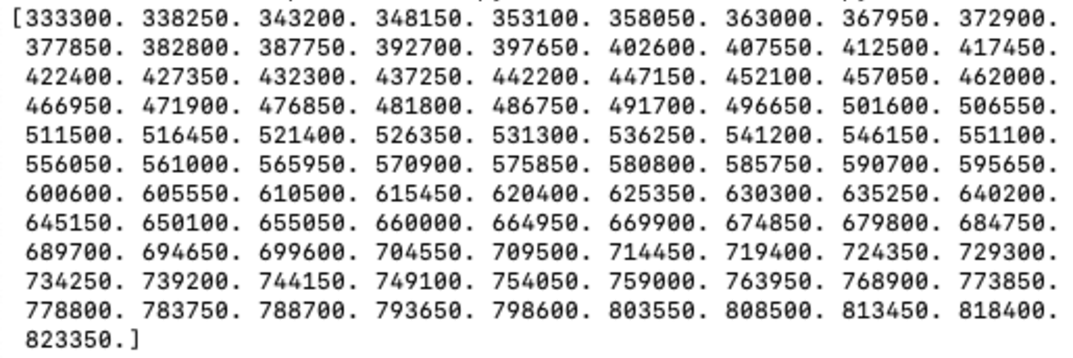
\includegraphics[width=.4\linewidth]{kadai1_1ans.pdf}
\hspace*{1mm}
\caption{課題1答え}
\end{center}
\end{figure}


\section{課題2}
課題2では$T$という行列が与えられており、$x(t), t = 0,1,2,\ldots,$が定義されている。初期値$x(0)$、$x(t)$それぞれが以下のように定義されている時の$t = 0 ~ 50$までの三次元ベクトルのそれぞれの値をグラフで表す問題である。これの答えは下の図にまとめる。
\[
  T = \left(
    \begin{array}{cccc}
      6 & -3 & -7 \\
      -1 & 2 & 1 \\
      5 & -3 & -6
    \end{array}
  \right) ,x(0) = \left(
    \begin{array}{cccc}
      4 \\
      0 \\
      3
    \end{array}
  \right),x(t + 1) = \frac{1}{\parallel Tx(t)\parallel}Tx(t)
\]

 
 
 
 
 
 
 

\begin{figure}[h]
\begin{center}
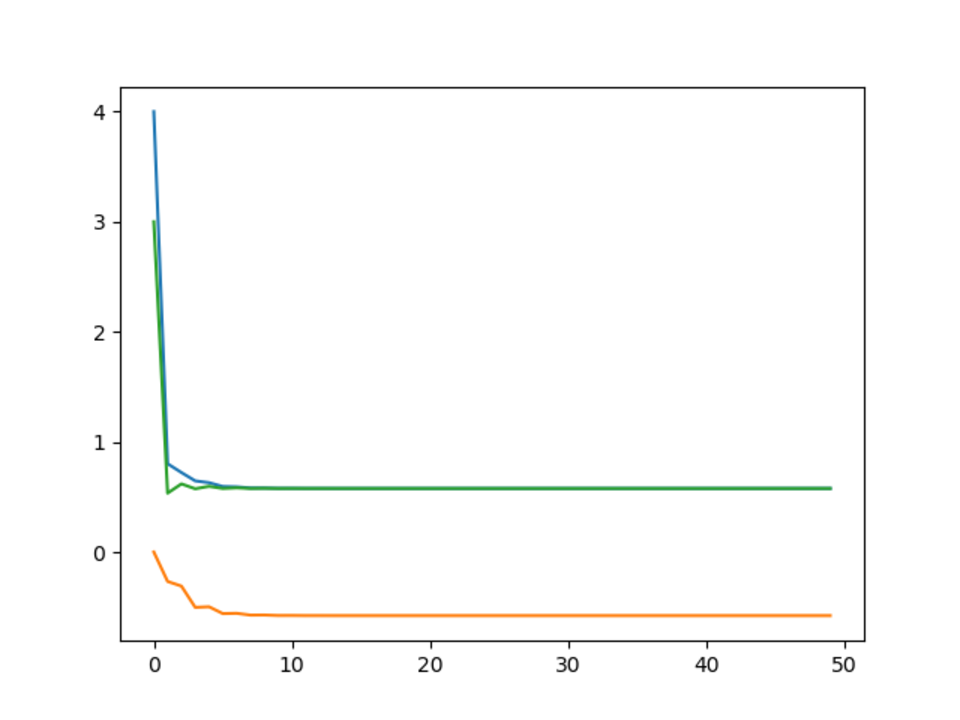
\includegraphics[width=.4\linewidth]{kadai1_2ans.pdf}
\hspace*{1mm}
\caption{課題2答え}
\end{center}
\end{figure}

\section{ソースコード}
 
 
 
 
 
 
 
 
  
\lstinputlisting[language=Python]{kadai1.py}

\end{document}


